% % !TeX program = xelatex
% !TeX spellcheck = es_ES
% !TeX encoding = utf8

\documentclass[onecolumn,10pt,titlepage,a4paper]{article}

\usepackage[a4paper,top=2.5cm,bottom=2cm,left=2cm,right=2cm,marginparwidth=1.75cm,headheight=28pt]{geometry}
% Formateo para castellano
%\usepackage[utf8]{inputenc}
\usepackage[spanish,mexico]{babel}
%\usepackage{natbib}


\newcommand{\celsius}{^\circ \mathrm{C}}
\newcommand{\air}{{\mathrm{humo}}}
%Bibliografía

% Simbolos para notas de pie
\usepackage[symbol]{footmisc}
\renewcommand*{\thefootnote}{\fnsymbol{footnote}}

% \renewcommand{\thefootnote}{\fnsymbol{footnote}}
% \footnote[num]{text}

% \pagestyle{myheading}
% \markright{Mi Documento \hfill Mi nombre \hfi}
%
\usepackage{fancyhdr,framed}
\setlength{\headheight}{15.2pt}
\pagestyle{fancy}
\lhead{Elementos Finitos II - 31.92 \\ Patricio Whittingslow -- 55423}
\chead{TP 2}


%\usepackage{subcaption}

% Para el entorno align


% Multiples columnas para glosario
\usepackage{multicol}

%Figuras y subtitulos
\usepackage{graphicx}
\usepackage{caption,subcaption}
\usepackage{hyperref}
\hypersetup{
    colorlinks,
    citecolor=black,
    filecolor=black,
    linkcolor=black,
    urlcolor=black
}
\usepackage[utopia,expert]{mathdesign} %Opcion "expert" para no romperme las smallcaps de helvetica. 
\usepackage{amsmath}

\newcommand{\rmfont}[1]{{\fontfamily{ptm}\selectfont%
		#1}}
\newcommand{\rmfontbf}[1]{{\fontfamily{ptm}\selectfont%
		\textbf{#1}}}
\newcommand{\rmfontsc}[1]{{\fontfamily{ptm}\selectfont%
		\textsc{#1}}}
    
\newcommand{\Matlab}{\rmfont{\sc Matlab}}
    \newcommand{\Adina}{{\sc ADINA}}
    \newcommand{\refp}[1]{(\ref{#1})}
    \newcommand{\unspace}{\!\!\!\!\!\!\!\!\!\!\!\!\!\!\!\!\!\!\!\!}
    \newcommand{\ms}{\ \ \ } %Matrix Spacing
    \newcommand{\di}{\textrm{d}}
    \newcommand{\jac}{\rmfontbf{J}}
    \newcommand{\Djac}{|\;\jac\;|}
    \newcommand{\dNi}{\di N_i}
    \newcommand{\sigmab}{\boldsymbol{\sigma}}
    \newcommand{\varepsilonb}{\boldsymbol{\varepsilon}}
    \newcommand{\Phib}{\boldsymbol{\Phi}}
    \newcommand{\CPhi}{\boldsymbol{\{ } \Phi \boldsymbol{\} }}
    \newcommand{\Mme}[1]{\boldsymbol{[}\mathbf{#1} \boldsymbol{]}}
    \newcommand{\Rme}[1]{\boldsymbol{\lfloor}\mathbf{#1} \boldsymbol{\rfloor}}
    \newcommand{\Cme}[1]{\boldsymbol{\{ }\mathbf{#1} \boldsymbol{\}} }
    \newcommand{\MB}{\Mme{B}}
    \newcommand{\MN}{\Mme{N}}
    \newcommand{\ME}{\Mme{E}}
    \newcommand{\Mk}{\Mme{k}}
    \newcommand{\MA}{\Mme{A}}
    \newcommand{\radial}{r}
    \newcommand{\eff}{f}
%Helvetica
\renewcommand{\familydefault}{\sfdefault}
\usepackage[scaled=1]{helvet}
\usepackage[format=plain,
            labelfont={bf,it},
            textfont=it]{caption}
%\usepackage[T1]{fontenc}
%--------------------------------------


\usepackage{siunitx}
\newcommand{\glossentry}[2]{$#1\ $ \indent #2 \par \vspace{.4cm} }
\newcommand{\adm}{\textrm{adm}}
\renewcommand\thepart{\Alph{part}}

\title{Informe Técnico - ITBA}

\author{Patricio Whittingslow}
%========================> Comienza Documento
\begin{document}
\begin{titlepage}
	\centering
	
	{ \large Instituto Tecnológico de Buenos Aires  \par }
	\vspace{2cm}
	{\Large \scshape Elementos Finitos II - 31.92 \par}
	\vspace{2cm}
	{\Huge \scshape Estudio técnico de un satélite de titanio utilizando el método de elementos finitos\par }
	\vspace{.5cm}
	{\Large  \par}
	\vspace{2cm}
	{\large \bf Autor \par}
	\vspace{.5cm}
	\textsc{\large Patricio Whittingslow -- 55423}
	\vspace{2cm}
	{\par \large Fecha de realización: \today \par}
	\vspace{1cm}
	{\large Fecha de entrega: .......................................\par}
	\vspace{\fill}
	{\large Firma del docente: .......................................}
	\vspace{\fill}
	\begin{figure}[htb!]
		\centering
		
\includegraphics[width=6cm]{fig/logoitba.png}
	\end{figure}
\end{titlepage}




\begin{multicols}{2}
	\section*{Glosario}
	\glossentry{\Cme{R}}{Vector de cargas térmicas.}
	\glossentry{\Mme{K}}{Matriz de conductividad.}
	\glossentry{\Mme{C}}{Matriz de capacidad térmica.}
	\glossentry{\Cme{T}}{Vector de Temperaturas.}
\end{multicols}

%\setcounter{section}{-1}

%\tableofcontents

\section*{Objetivo}
Se va efectuar un pequeño estudio térmico de un satélite ubicado en el espacio profundo. El problema será resuelto mediante el método de elementos finitos y se analizaran las limitaciones de la resolución.

\section*{Hipótesis}
\begin{itemize}
	\item Material isótropo y homogéneo
	\item Propiedades sin dependencia de variables termodinámicas
\end{itemize}


\section*{Método}

El satélite será modelado como un cubo de titanio macizo. Este se encuentra en el vacío del espacio profundo, el cual tiene una temperatura $T_{\mathrm{CMBR}}=2,7$ K. El modelo se simplifica tomando solo una octava parte del satélite, aprovechando la doble simetría. 

El satélite tiene lados de longitud $L=0,8$m. Las propiedades del titanio son las siguientes:
\begin{itemize}
	\item $c_p = 528 \si{\joule \per \kilogram \per \kelvin}$
	\item $\rho = 4500\si{\kilogram \per \meter \cubed }$
	\item $k = 17 \si{\watt \per \meter \kelvin}$
\end{itemize}

Las condiciones de operación son las siguientes
\begin{itemize}
	\item El centro del satélite opera a 300K.
	\item El satélite genera $q_{G}=2\si{\kilo \watt \per \meter \cubed}$
	\item El calor radiado tomando en cuenta el factor de forma queda $q_{r}=\SI{1,417e-8}{\watt \per \meter \squared \per \kelvin^4} \cdot \left( T^4 - T^4_{\mathrm{CMBR}} \right)$
\end{itemize}

Para la resolución se dividió el satélite en 64 elementos H8. 

Las condiciones de borde son las siguientes
\begin{itemize}
	\item Se fija el punto central del satélite a 300K
	\item Las superficies expuestas del satélite intercambian calor con el entorno según la ecuación mencionada anteriormente
\end{itemize}
Se comienza la iteración fijando las temperaturas en 300 grados kelvin y termina la iteración una vez llegado a un error aceptable (ecuación \ref{ec:error})
\begin{equation}\label{ec:error}
	e_{\mathrm{convergencia}}=\frac{||\CT^{n+1}-\CT^{n}||}{||\CT^{n}||} < 10^{-8}
\end{equation}

\section*{Resultados}
Se puede observar en la figura \ref{fig:Convergencia} como la solución converge tal que la superficie es más caliente que el interior del satélite.


\begin{figure}[htb!]
	\centering
	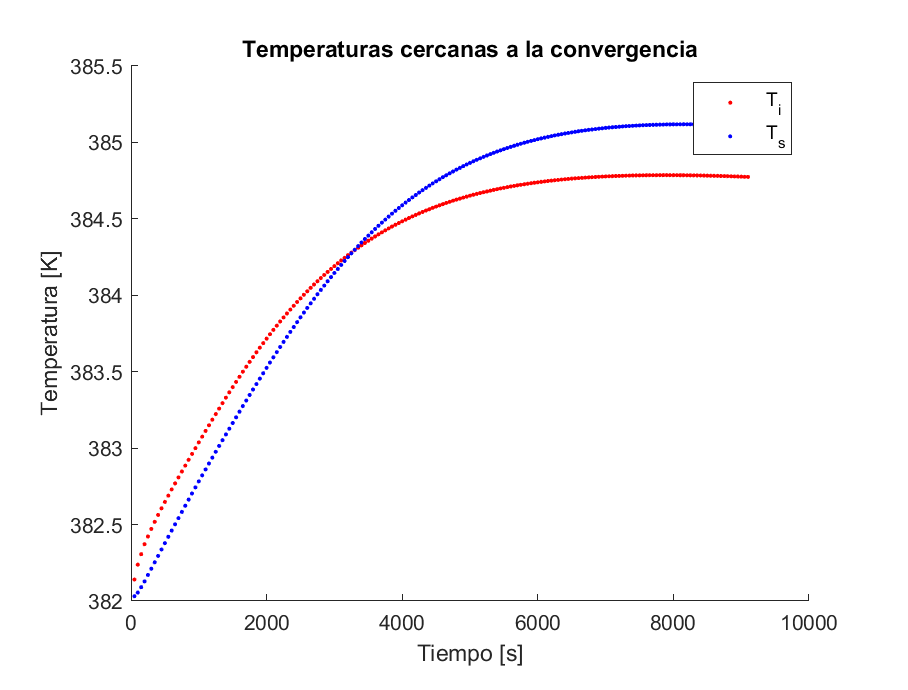
\includegraphics[width=0.8\textwidth]{fig/convergenciadiv9.eps}
	\caption{Evolución de temperaturas. $T_s$ es la temperatura de la superficie radiante. $T_i$ es la temperatura del nodo interior vecino a la superficie (central a la superficie).}
	\label{fig:Convergencia}
\end{figure}


\begin{figure}[htb!]
	\centering
	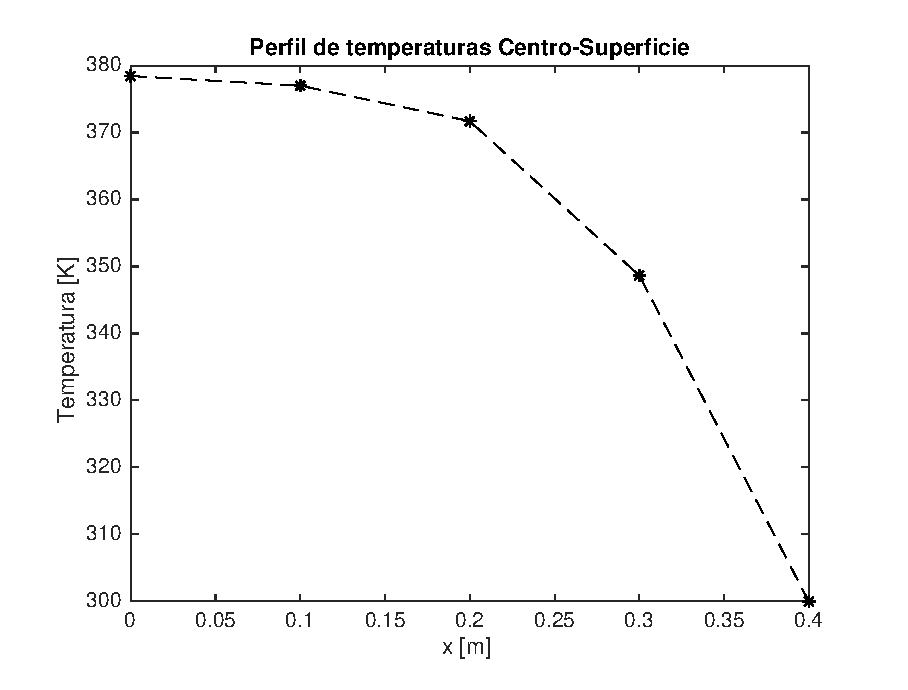
\includegraphics[width=0.8\textwidth]{fig/perfil9div.eps}
	\caption{$x=0,4$m es el centro del satélite y $x=0$m es la superficie.}
	\label{fig:perfilinterior}
\end{figure}

\begin{figure}[htb!]
	\centering
	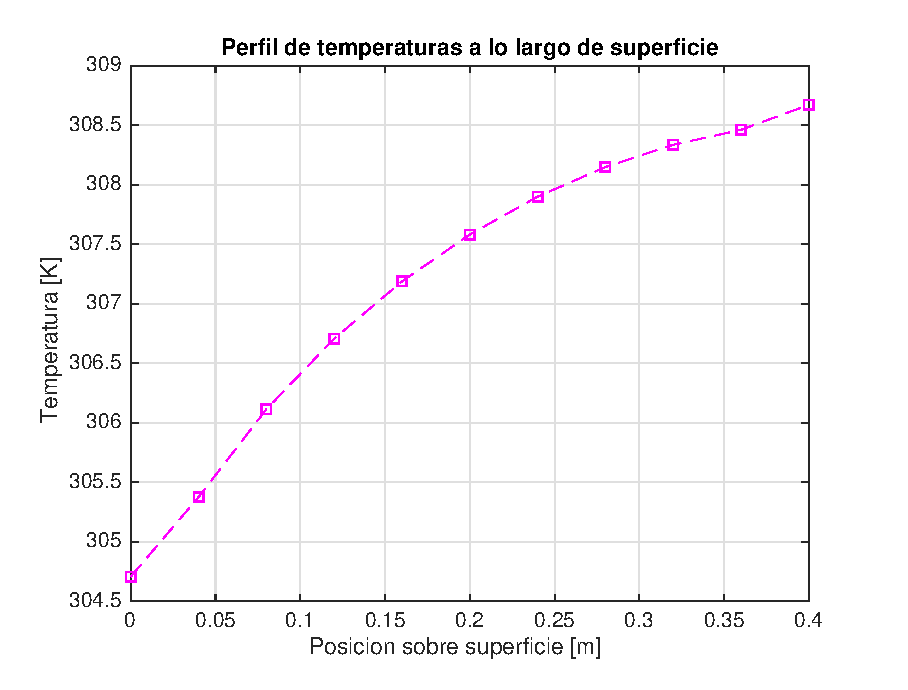
\includegraphics[width=0.8\textwidth]{fig/perfilRad9div.eps}
	\caption{$x=0,4$m es en el borde del satélite y $x=0$m es en el centro de la superficie.}
	\label{fig:perfilsuperficie}
\end{figure}

%\bibliography{labibliografia} % Indica archivo
%\bibliographystyle{plainnat} 

\end{document}